\documentclass[../../main.tex]{subfiles}
\begin{document}

{\bf [解]}
題意の楕円と円を$C: \dfrac{x^2}{4}+\dfrac{y^2}{3}=1$，$C_1: (x-1)^2+y^2=1$，$C_2: (x+1)^2+y^2=1$とおく．
対称性から$P$が$x\ge0$にあるとして良い．$P$を$C$上のこの範囲内で$P(X,Y)$と固定して$R,Q$をうごかす．

\begin{figure}[htb]
 \begin{center}
  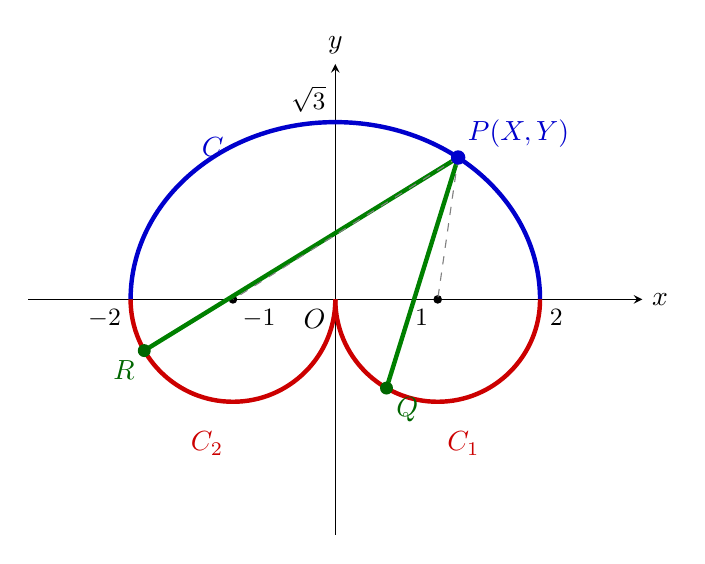
\begin{tikzpicture}[scale=1.3, >=stealth]

  % --- 1. 座標軸 ---
  \draw[->, thin] (-3.0,0) -- (3.0,0) node[right] {$x$};
  \draw[->, thin] (0,-2.3) -- (0,2.3) node[above] {$y$};
  \node[below left] at (0,0) {$O$};

  % --- 2. 楕円 C および 円 C_1, C_2 (普通の線 `thin`) ---
  % 楕円 C : x^2/4 + y^2/3 = 1 (a=2, b=sqrt(3) ≒ 1.732)
  % \draw[thin, blue!80!black] (0,0) ellipse (2 and 1.732);
  \draw[ultra thick, blue!80!black] (2,0) arc (0:180:2 and 1.732);
  \node[blue!80!black, above right] at (-1.4, 1.3) {$C$};

  % 円 C_1 : (x-1)^2 + y^2 = 1
  % \draw[thin, red!80!black] (1,0) circle (1);
  % 円 C_1 上半円 (y >= 0): 普通の線 (thin)
  %\draw[thin, red!80!black] (2,0) arc (0:180:1);

  % 円 C_1 下半円 (y <= 0): 太線 (ultra thick)
  \draw[ultra thick, red!80!black] (2,0) arc (360:180:1);
  \node[red!80!black, below right] at (1,-1.2) {$C_1$};

  % 円 C_2 : (x+1)^2 + y^2 = 1
  %\draw[thin, red!80!black] (-1,0) circle (1);
  % 円 C_2 上半円 (y >= 0): 普通の線 (thin)
  %\draw[thin, red!80!black] (0,0) arc (0:180:1);

  % 円 C_2 下半円 (y <= 0): 太線 (ultra thick)
  \draw[ultra thick, red!80!black] (0,0) arc (360:180:1);
  \node[red!80!black, below left] at (-1,-1.2) {$C_2$};

  % --- 3. 焦点 F_1(1,0), F_2(-1,0) ---
  \coordinate (F1) at (1,0);
  \coordinate (F2) at (-1,0);

  \fill[black] (F1) circle (1.2pt) node[below left, font=\small] {$1$};
  \fill[black] (F2) circle (1.2pt) node[below right, font=\small] {$-1$};

  % --- 4. 点 P(X,Y) と 最大にならない一般の点 Q, R の設定 ---
  % 点 P (第一象限: X = 1.2)
  \coordinate (P) at (1.2, 1.386);

  % 点 Q: F_1 を通らない一般の位置 (例: C_1 上の theta = 240度 付近)
  \coordinate (Q) at ({1 + cos(240)}, {sin(240)}); % (0.5, -0.866)

  % 点 R: F_2 を通らない一般の位置 (例: C_2 上の theta = 210度 付近)
  \coordinate (R) at ({-1 + cos(210)}, {sin(210)}); % (-1.866, -0.5)

  % --- 5. 線分 PQ, PR の描画 (ここだけを太字/太線 `ultra thick` に指定) ---
  \draw[ultra thick, green!50!black] (P) -- (Q);
  \draw[ultra thick, green!50!black] (P) -- (R);

  % 参考: P と F1, F2 を結ぶ補助線 (破線)
  \draw[dashed, gray] (P) -- (F1);
  \draw[dashed, gray] (P) -- (F2);

  % --- 6. 各点のプロットとラベル ---
  \fill[blue!80!black] (P) circle (2pt) node[above right] {$P(X,Y)$};
  \fill[green!40!black] (Q) circle (1.8pt) node[below right] {$Q$};
  \fill[green!40!black] (R) circle (1.8pt) node[below left] {$R$};

  % --- 7. 目盛りラベル ---
  \node[below left, font=\small] at (-2,0) {$-2$};
  \node[below right, font=\small] at (2,0) {$2$};
  \node[above left, font=\small] at (0,1.732) {$\sqrt{3}$};

\end{tikzpicture}
\caption{楕円$C, C_1,C_2$および$L,M,N$の様子}
 \end{center}
\end{figure}

まず線分$PQ$について考える．以下$s=\sin\theta,\ c=\cos\theta$と書くことにすると $Q$は$C_1$の上にあるから$Q(1+c,s)\ (\pi\le\theta\le2\pi)$とおけて，
\begin{align}
\begin{split}
|PQ|^2
 &=(1+c-X)^2+(s-Y)^2 \\
 &=(1+c)^2+s^2+X^2+Y^2-2X(1+c)-2Ys \\
 &=X^2+Y^2-2(X-1) -2(X-1)c-2Ys \\
 &=X^2+Y^2-2(X-1) - 2\begin{pmatrix}X-1\\Y\end{pmatrix}\cdot\begin{pmatrix}c\\s\end{pmatrix}
\end{split}
\end{align}
とかける．$F_1(1,0)$とおくと
\begin{align}
 |PQ|^2 = X^2+Y^2-2(X-1) - 2 \overrightarrow{F_1P}\cdot \overrightarrow{F_1Q}
\end{align}
である．従って第4項の内積が最小の時に$|PQ|^2$は最大になるが，これは$\overrightarrow{FP}$と$\overrightarrow{FQ}$のなす角度が$\pi$の時，すなわち線分$PQ$が$F_1$を通る時に最小になる．従って$|PQ|>0$と合わせて$|PQ|$が最大になるのは線分$PQ$が$F_1$を通る時である．

\begin{figure}[htb]
 \begin{center}
  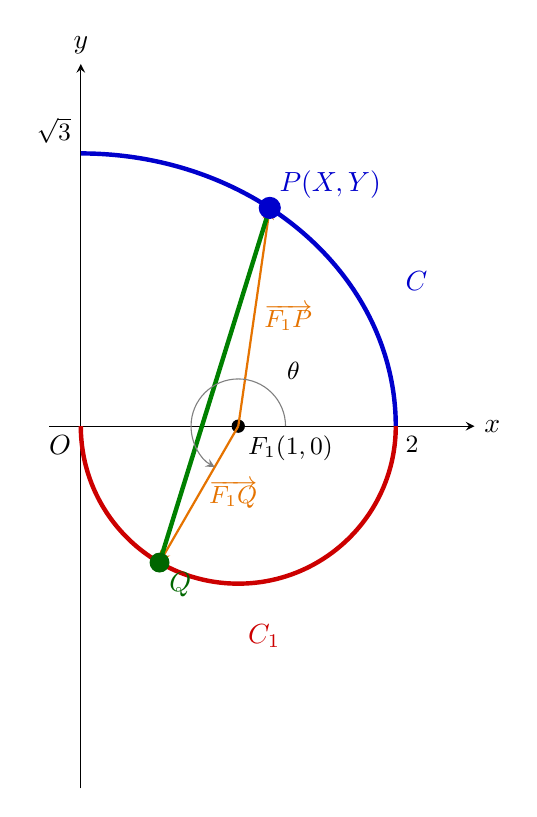
\begin{tikzpicture}[scale=2, >=stealth]

  % --- 1. 座標軸 ---
  \draw[->, thin] (-0.2,0) -- (2.5,0) node[right] {$x$};
  \draw[->, thin] (0,-2.3) -- (0,2.3) node[above] {$y$};
  \node[below left] at (0,0) {$O$};

  % --- 2. 楕円 C および 円 C_1 ---
  % 楕円 C : 第一象限の弧
  \draw[ultra thick, blue!80!black] (2,0) arc (0:90:2 and 1.732);
  \node[blue!80!black, above right] at (2, 0.8) {$C$};

  % 円 C_1 : 下半円 (y <= 0)
  \draw[ultra thick, red!80!black] (2,0) arc (360:180:1);
  \node[red!80!black, below right] at (1,-1.2) {$C_1$};

  % --- 3. 焦点 F_1(1,0) ---
  \coordinate (F1) at (1,0);
  \fill[black] (F1) circle (1.2pt) node[below right, font=\small] {$F_1(1,0)$};

  % --- 4. 点 P(X,Y) と 点 Q の設定 ---
  % 点 P (第一象限: X = 1.2)
  \coordinate (P) at (1.2, 1.386);

  % 点 Q (例: theta = 240度)
  \coordinate (Q) at ({1 + cos(240)}, {sin(240)}); % (0.5, -0.866)

  % --- 5. ベクトル F_1P, F_1Q の描画 (矢印付き) ---
  % F_1 -> P ベクトル
  \draw[->, thick, orange!90!black] (F1) -- (P) node[midway, right, font=\small] {$\overrightarrow{F_1P}$};

  % F_1 -> Q ベクトル
  \draw[->, thick, orange!90!black] (F1) -- (Q) node[midway, right, font=\small] {$\overrightarrow{F_1Q}$};

  % 線分 PQ (緑太線)
  \draw[ultra thick, green!50!black] (P) -- (Q);

  % --- 6. 角度 theta の描画 (F1 を中心とする偏角) ---
  % x 軸正の向き(0度)から Q の方向(240度)への角
  \draw[->, thin, gray] (1.3,0) arc (0:240:0.3);
  \node[font=\small] at (1.35, 0.35) {$\theta$};

  % --- 7. 各点のプロットとラベル ---
  \fill[blue!80!black] (P) circle (2pt) node[above right] {$P(X,Y)$};
  \fill[green!40!black] (Q) circle (1.8pt) node[below right] {$Q$};

  % --- 8. 目盛りラベル ---
  \node[below right, font=\small] at (2,0) {$2$};
  \node[above left, font=\small] at (0,1.732) {$\sqrt{3}$};

\end{tikzpicture}
\caption{$F_1P$および$F_1Q$の様子}
 \end{center}
\end{figure}


全く同様に考えると，点$R$については線分$PR$が$F_2(-1,0)$を通る時に$|PR|^2$が最大になる．

従って，点$P$を固定した時の$|PQ|+|PR|$の最大値は円$C_1,C_2$の半径が1だから
\begin{align}
\max(|PQ|+|PR|)
 &=|PF_1|+|PF_2|+2 \\
\end{align}
となる．さらに$C$は$c$は長軸$4$の楕円で，$F_1,F_2$がこの楕円の焦点だから$P$にかかわらず$|PF_1|+|PF_2|=4$で一定である．
従って
\begin{align}
 \max(|PQ|+|PR|) = 4+2=6
\end{align}
である．

\begin{figure}[htb]
\begin{center}
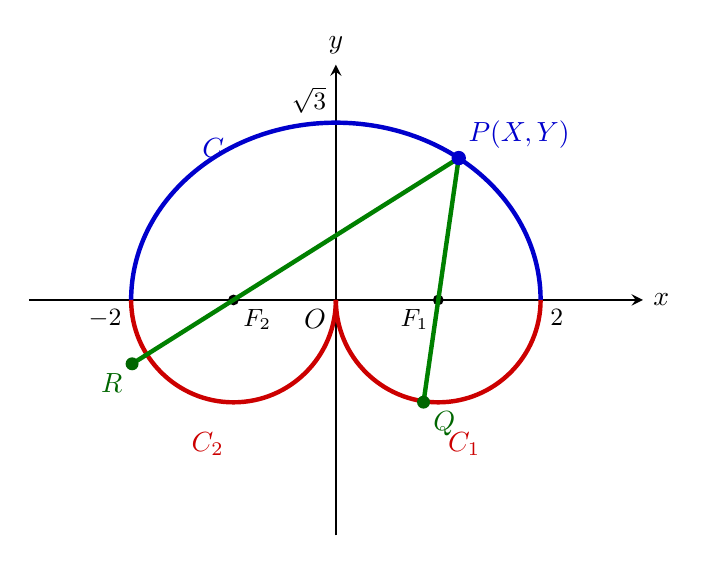
\begin{tikzpicture}[scale=1.3, >=stealth]

  % --- 1. 座標軸 ---
  \draw[->, thick] (-3.0,0) -- (3.0,0) node[right] {$x$};
  \draw[->, thick] (0,-2.3) -- (0,2.3) node[above] {$y$};
  \node[below left] at (0,0) {$O$};


  % --- 2. 楕円 C および 円 C_1, C_2 (普通の線 `thin`) ---
  % 楕円 C : x^2/4 + y^2/3 = 1 (a=2, b=sqrt(3) ≒ 1.732)
  % \draw[thin, blue!80!black] (0,0) ellipse (2 and 1.732);
  \draw[ultra thick, blue!80!black] (2,0) arc (0:180:2 and 1.732);
  \node[blue!80!black, above right] at (-1.4, 1.3) {$C$};

  % 円 C_1 : (x-1)^2 + y^2 = 1
  % \draw[thin, red!80!black] (1,0) circle (1);
  % 円 C_1 上半円 (y >= 0): 普通の線 (thin)
  %\draw[thin, red!80!black] (2,0) arc (0:180:1);

  % 円 C_1 下半円 (y <= 0): 太線 (ultra thick)
  \draw[ultra thick, red!80!black] (2,0) arc (360:180:1);
  \node[red!80!black, below right] at (1,-1.2) {$C_1$};

  % 円 C_2 : (x+1)^2 + y^2 = 1
  %\draw[thin, red!80!black] (-1,0) circle (1);
  % 円 C_2 上半円 (y >= 0): 普通の線 (thin)
  %\draw[thin, red!80!black] (0,0) arc (0:180:1);

  % 円 C_2 下半円 (y <= 0): 太線 (ultra thick)
  \draw[ultra thick, red!80!black] (0,0) arc (360:180:1);
  \node[red!80!black, below left] at (-1,-1.2) {$C_2$};

  % --- 4. 焦点 F_1(1,0), F_2(-1,0) ---
  \coordinate (F1) at (1,0);
  \coordinate (F2) at (-1,0);

  \fill[black] (F1) circle (1.5pt) node[below left, font=\small] {$F_1$};
  \fill[black] (F2) circle (1.5pt) node[below right, font=\small] {$F_2$};

  % --- 5. 点 P(X,Y) の設定 (第一象限の例: X=1.2) ---
  % Y = sqrt(3 * (1 - 1.2^2 / 4)) ≒ 1.386
  \coordinate (P) at (1.2, 1.386);

  % --- 6. 最大値を与える点 Q_max, R_max (P, F1/F2 を通る直線と円の交点) ---
  % P -> F1 のベクトル方向に延ばして円 C_1 の下側境界と交わる点 Q
  % P -> F2 のベクトル方向に延ばして円 C_2 の下側境界と交わる点 R
  
  % P-F1 の傾きから Q の座標を計算 (F1 からの距離 1)
  \path (P) -- (F1) coordinate[pos=1.72] (Q);
  % P-F2 の傾きから R の座標を計算 (F2 からの距離 1)
  \path (P) -- (F2) coordinate[pos=1.45] (R);

  % --- 7. 線分 PQ, PR (最大時の線分) の描画 ---
  % 線分 PF1 + F1Q = PQ (直線)
  \draw[ultra thick, green!50!black] (P) -- (Q);
  \draw[ultra thick, green!50!black] (P) -- (R);

  % --- 8. 各点のプロットとラベル ---
  \fill[blue!80!black] (P) circle (2pt) node[above right] {$P(X,Y)$};
  \fill[green!40!black] (Q) circle (1.8pt) node[below right] {$Q$};
  \fill[green!40!black] (R) circle (1.8pt) node[below left] {$R$};

  % --- 9. 目盛りラベル ---
  \node[below left, font=\small] at (-2,0) {$-2$};
  \node[below right, font=\small] at (2,0) {$2$};
  \node[above left, font=\small] at (0,1.732) {$\sqrt{3}$};

\end{tikzpicture}
\caption{$|PQ|+|PR|$が最大の時の様子．}
\end{center} 
\end{figure}



\newpage

\end{document}
